% vim: filetype=tex spell

%Background Chapter : Recount the work that crank did

\chapter{Background}

\label{ch:BG}

%NOTE: this wording is similar to Crank 1.6

The \ac{LPMT} was originally designed in 1971 by Dr. Michael Polites\cite{Polites71}. It was refined into a stabilization system by Dr. Donald Mentch for his masters degree in 2003 and further refined into a system for the \ac{ARC} as his doctoral work in 2011\cite{Mentch11}. The system described in \cite{Mentch11} proposes a concept for 3-axis stabilization that is valid for a nearly circular and nearly polar Earth-orbiting satellite.

\section{\aclp{LPMT}}

The \ac{ARC} \ac{ACDS} uses \acfp{LPMT} to create the torque needed to properly orient the CubeSat. The torque equation for all magnetic torquers, including the \acp{LPMT}, is shown in \cref{eq:magtorque} where $\vec{m}$ is the magnetic dipole moment of the torquer and $\vec{B}$ is the local magnetic field. The torque produced is always perpendicular to the magnetic field and the dipole moment. Also the component of $\vec{m}$ that is perpendicular to $\vec{B}$ is the only component that produces torque.

\begin{equation}
    \vec{\tau} = \vec{m} \cross \vec{B}
    \label{eq:magtorque}
\end{equation}

Other CubewSats have used magnetic torque rods and coils are governed by the same equation. The unique part about \acp{LPMT} is that the magnetic dipole moment comes from the core of the torquer and does not depend on a continuous current flow to create torque.


\subsection{Hard Magnetic Core}

The cores of the \acp{LPMT} are made of a hard magnetic material that ideally have a saturation curve that looks like \cref{fig:histlpmt}. The hysteresis curve shows the response of the torquer,$M$, with respect to the driving force, H, which is proportional to the current through the solenoid. The response of the torquer depends on the driving force as well as the previous state of the torquer so that when there is no driving force the torquer response has two possible states depending on how the torquer was last driven. The \ac{LPMT} operates by switching the cores between these saturation points, $M_s$ and $-M_s$. The \ac{LPMT} cores are driven to saturation using a capacitor to provide a current pulse through a solenoid surrounding the magnetic core. Even after current stops flowing through the solenoid the core will have a dipole moment of $\pm M_r$ depending on which direction the current was run in \cite{Mentch11}.

\begin{figure}[H]
    \centering
    \begin{tikzpicture}

    \def\Ms{2.0}
    \def\Hs{1.8}
    %draw axis
    \draw[<->] (-\Hs-0.5,0) -- (\Hs+0.5,0);
    \draw[<->] (0,-\Ms-0.5) -- (0,\Ms+0.5);

    %black lines that point back to the origin
    \draw[->] (\Hs,\Ms) -- (\Hs,0);
    \draw[->] (-\Hs,-\Ms) -- (-\Hs,0);
    
    %draw axis lables
    \draw (0,\Ms+0.25) node[anchor=east] {$M$};
    \draw (\Hs+0.25,0) node[anchor=north] {$H$};

    %green lines, magnetization in one direction
    \draw[->,green,very thick] (0,\Ms) -- (-0.2,\Ms);
    \draw[->,green,very thick] (-0.2,\Ms) -- (-\Hs,-\Ms);
    \draw[->,green,very thick] (-\Hs-0.7,-\Ms) -- (0,-\Ms);

    %yellow lines, magnetization in the other direction
    \draw[->,blue,very thick] (0,-\Ms) -- (0.2,-\Ms);
    \draw[->,blue,very thick] (0.2,-\Ms) -- (\Hs,\Ms);
    \draw[->,blue,very thick] (\Hs +0.7,\Ms) -- (0,\Ms);

    %draw lables
    \draw (-\Hs,-\Ms) node[anchor=north] {$-M_s$};
    \draw (\Hs,\Ms) node[anchor=south] {$M_s$};

    \draw (-\Hs,0) node[anchor=north east] {$-H_s$};
    \draw (\Hs,0) node[anchor=south west] {$H_s$};

    \draw (0,-\Ms) node[anchor=south east] {$-M_r$};
    \draw (0,\Ms) node[anchor=north west] {$M_r$};


    \end{tikzpicture}
    \caption{Hysteresis loop for an ideal hard magnetic material}
    \label{fig:histlpmt}
\end{figure}

\subsection{Torquer Pair}

%TODO: add discussion of position (in)dependence of torquer par torque

The cores of the \acp{LPMT} are driven to saturation in the direction of the rod. This gives two possible states for each rod. Because in both states the rod generates a net dipole moment, the rods are operated in pairs so that three possible dipole moments can be produced as shown in \cref{fig:moments}, where M is the dipole moment of a single torquer.

\begin{figure}[H]
    \centering
    \begin{tikzpicture}
    \def\L{1.5}     %define arrow length
    \draw[->,red,very thick] (1  , 0) -- (1  ,\L);
    \draw[->,red,very thick] (1.5, 0) -- (1.5,\L);
    \draw (1.25,-0.5) node {+2M};

    \draw[->,red,very thick] (3  ,\L) -- (3  , 0);
    \draw[->,red,very thick] (3.5, 0) -- (3.5,\L);
    \draw (3.25,-0.5) node {0M};

    \draw[->,red,very thick] (5  ,\L) -- (5  , 0);
    \draw[->,red,very thick] (5.5,\L) -- (5.5, 0);
    \draw (5.25,-0.5) node {-2M};
    \end{tikzpicture}
    \caption{Possible dipole moments for a torquer pair}
    \label{fig:moments}
\end{figure}

Because each \ac{LPMT} pair can only produce three distinct values of dipole moment, the output of a \ac{LPMT} algorithm must be quantized. \Cref{fig:lpmtq} shows the quantization function for two torquers, where $M_{command}$ is the commanded dipole moment from the algorithm and $M_{command_q}$ is the quantized dipole moment that takes on one of the values that the torquers can produce.

\begin{figure}[H]
    \centering
    \begin{tikzpicture}

    \draw[<->,green,very thick] (2,2) -- (1,2) -- (1,0) -- (-1,0) -- (-1,-2) -- (-2,-2);

    %draw axis
    \draw[<->] (-3,0) -- (3,0);
    \draw[<->] (0,-3) -- (0,3);

    %draw axis labels
    \draw (0,3) node[anchor=south] {$M_{command_q}$};
    \draw (3,0) node[anchor=west] {$M_{command}$};

    \draw (2,0)  node[anchor=north] {$+2M$};
    \draw (1,0)  node[anchor=north] {$+1M$};
    \draw (-1,0) node[anchor=south] {$-1M$};
    \draw (-2,0) node[anchor=south] {$-2M$};

    \draw (0,2)  node[anchor=east] {$+2M$};
    \draw (0,-2) node[anchor=west] {$-2M$};

    \end{tikzpicture}
    %\caption{Quantization function for \acs*{LPMT}\protect\nocite{Mentch11}}
    \caption{Quantization function for \acs*{LPMT}}
    \todo[inline]{Figure reproduced from Crank}
    \label{fig:lpmtq}
\end{figure}

\subsection{Torquer Sets}

For the initial design in \cite{Mentch11} it was proposed to use a 10 second torquer flipping interval and two pairs of different torquers in each axis. One pair, called the primary torquers, was made of Alnico1 and had a dipole moment of $0.022~\unit{A}{\cdot}\unit{m^2}$. This pair was to be used for the detumble phase where a larger dipole moment allows for more torque to slow the satellite faster. For the alignment phase the second set of torquers, the vernier torquers, were proposed. The vernier torquers were to have a dipole moment of $0.00011~\unit{A}{\cdot}\unit{m^2}$.

\section{Detumble Algorithm (Mode 1)}

The purpose of the detumble algorithm is to reduce the initial tipoff rates. When CubeSats are ejected from the \ac{PPOD} significant rotation rates can be induced\todo{find reference}.

To detumble \ac{ARC} the control law shown in \cref{eq:crossl} is used. This is used by many CubeSats with conventional torquers to detumble\todo{find reference}. The significant difference in this case is that the magnetic dipole moment will be quantized due to the \acp{LPMT}.

\begin{equation}
    \vect{m}_{command} = k {\frac{\vect{\omega}_{error} \cross \dot{\vect{B}}}{\vect{B} \cdot \vect{B}}}
    \label{eq:crossl}
\end{equation}

The original simulation transitioned to detumble once the rotation rate error was less than $0.002~\unit{\frac{rad}{sec}}$, corresponding to about 1.7 revolutions/orbit. It was later suggested that the transition could run for a pre-determined time that was more than sufficient to detumble the satellite.

\section{Alignment Algorithm}

The job of the alignment algorithm is to align the \ac{ARC} in the proper attitude and maintain this attitude for the rest of the mission. This is achieved using bias windows as shown in \cref{fig:windows}. In the equatorial windows the magnetic field is nearly parallel to the surface of the Earth and in the polar window the magnetic field is nearly perpendicular to the surface of the Earth. By biasing the torquers in such a way as to line up the appropriate axis in each window, three-axis alignment can be achieved. There is no window at the south pole because the magnetic south pole is located far from the geographical south pole making it necessary to know the direction of approach to determine the window location.

\begin{figure}[H]
    \centering
    % vim: filetype=tex spell

\tikzstyle{winLbl} = [rectangle,text width=5em,text centered]

\newcommand{\cubesat}[2]{
    \draw (#1:#2) node{\pgftext[rotate=#1]{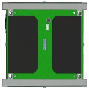
\includegraphics[height=7mm]{cube-icon}}};
}

%digram showing bias windows for the alignment algorithm

\begin{tikzpicture}


    \def\incline{90}                            % Orbit Inclination (degrees)
    \def\poleWindow{10}                         % Polar alignment windows in degrees
    \def\offset{10}                             % Amount the window is offset in the wake direction (i.e.  earlier) in degrees eq_window = 15;
    \def\eqWindow{15}                           % Equatorial alignment window in degrees
    %\def\latTrigger{\incline-\poleWindow}       % Corrects polar window for inclination angle
    \def\latTrigger{80}                         % Corrects polar window for inclination angle

    \def\winR{3cm}                                %window radius for drawing
    \def\axisLen{4cm}

    %import earth background
    \pgftext{
\includegraphics[height=4cm]{earth}}

    %draw orbit
    \draw[->,black,thin] (0,0) circle (\winR);

    %draw axis
    \draw[<->] (-\axisLen,0) -- (\axisLen,0);
    \draw[<->] (0,-\axisLen) -- (0,\axisLen);

    {
        \tikzset{>=triangle 45} %make a bigger arrow
        \draw[->] (25:\winR+0.5cm) arc (25:45:\winR+0.5cm);
        \draw[winLbl]   (35:\winR+0.5cm) node[anchor=south west] {\small Orbit Direction};
    }


    %draw bias windows
    %northbound equatorial window
    \draw[green]                    (0,0)  -- (\eqWindow/2 - \offset:\winR) arc (\eqWindow/2 - \offset:-\eqWindow/2 - \offset:\winR) -- cycle;
    \fill[nearly transparent,green] (0,0)  -- (\eqWindow/2 - \offset:\winR) arc (\eqWindow/2 - \offset:-\eqWindow/2 - \offset:\winR) -- cycle;

    \draw[green,winLbl] (-\offset:\winR+0.5cm) node[anchor=north west] {\small Northbound Equatorial Window};
    \cubesat{-\offset}{\winR}


    %south bound equatorial window
    \draw[red]                    (0,0)  -- (180-\eqWindow/2 - \offset:\winR) arc (180-\eqWindow/2 - \offset:180 +\eqWindow/2 - \offset:\winR) -- cycle;
    \fill[nearly transparent,red] (0,0)  -- (180-\eqWindow/2 - \offset:\winR) arc (180-\eqWindow/2 - \offset:180 +\eqWindow/2 - \offset:\winR) -- cycle;

    \draw[red,winLbl] (180-\offset:\winR+0.5cm) node[anchor=south east] {\small Southbound Equatorial Window};
    \cubesat{180-\offset}{\winR}


    %north polar window
    \draw[blue]                    (0,0)  -- (\latTrigger - \offset:\winR) arc (\latTrigger - \offset:90:\winR) -- cycle;
    \fill[nearly transparent,blue] (0,0)  -- (\latTrigger - \offset:\winR) arc (\latTrigger - \offset:90:\winR) -- cycle;

    \draw[blue,winLbl] (90-\poleWindow/2-\offset/2:\winR+0.5cm) node[anchor=south west] {\small North Polar Window};

    %draw CubeSat
    \cubesat{90-\poleWindow/2-\offset/2}{\winR}

    %draw axis labels
    \draw (0,\axisLen) node[anchor=south] {N};
    \draw (\axisLen,0) node[anchor=west] {E};

    \draw (0,-\axisLen) node[anchor=north] {S};
    \draw (-\axisLen,0) node[anchor=east] {W};

\end{tikzpicture}

    \caption{Bias windows for alignment mode}
    \label{fig:windows}
\end{figure}

\Cref{fig:windows} shows that the bias windows are offset so that they occur just before the equator or pole. The reason for this is shown in \cref{fig:winplace}. If the torquers are biased before the satellite passes over the vertical (or horizontal) field lines then the tendency is to rotate in the desired direction. If the torquers are biased afterwards then the tendency is to rotate the satellite opposite the desired direction.\cite{Mentch11}

\begin{figure}[htb!]
    \centering
    
    \begin{tikzpicture}
        \def\winR{4.5cm}                                %window radius for drawing
        \def\earthR{3.2cm}                              %earth radius for drawing
        \def\axlen{1.5cm}                               %axis length for drawing
        \def\favang{65}                                 %angle for favorable orientation
        \def\unfavang{115}                              %angle for unfavorable orientation
        \def\bias{35}                                   %half angle for bias arrows
        \def\ARCheight{15mm}

        \begin{scope}
            \clip (-\winR,2cm) rectangle (\winR,\winR+\axlen);

            %draw vertical field line
            \draw[color=blue,field] (0,\earthR) -- (0,\winR+\axlen);
            %draw "earth"
            \draw[color=green!60!black,very thick] (0,0) circle (\earthR);

            %draw favorable cubesat
            \cubesat{\favang}{\winR}
            \draw[bias] (\favang:\winR+0.5cm) ++(\favang-\bias:0.5cm) arc (\favang-\bias:\favang+\bias:0.5cm);
            \draw[motion] (\favang:\winR+1cm) ++(\favang-90:0.7cm) arc (\favang-90:\favang+90:0.7cm);

            %draw unfavorable cubesat
            \cubesat{\unfavang}{\winR}
            \draw[bias] (\unfavang:\winR+0.5cm) ++(\unfavang-\bias:0.5cm) arc (\unfavang-\bias:\unfavang+\bias:0.5cm);
            \draw[motion] (\unfavang:\winR+1cm) ++(\unfavang+90:0.7cm) arc (\unfavang+90:\unfavang-90:0.7cm);        %draw arrow in the other direction

        \end{scope}
        \draw (\unfavang:\winR) ++(\unfavang:\axlen+0.2cm) node[rotate=\unfavang-90,anchor=south] {\tiny Unfavorable};
        \draw (\favang:\winR) ++(\favang:\axlen+0.2cm) node[rotate=\favang-90,anchor=south] {\tiny Favorable};
    \end{tikzpicture}
    \caption{Bias window offset}
    \label{fig:winplace}
\end{figure}

\Cref{fig:winplace} is similar to Figure 29 in \cite{Mentch11}. The major change to note is that the axis definitions have been changed to match those of the \ac{ARC}.

\subsection{Mode 2}

Mode 2 is initiated at the end of the detumble phase. In mode 2 the torquers are biased as shown in \cref{fig:m2b} with the Y-axis torquers biased in the equatorial windows and the Z-axis torquers biased in the polar window. While the bias is active the algorithm in \cref{eq:crossl} is used to dampen out the oscillations caused by the bias. Outside the three bias windows all torquers are set to cancel each other and the \ac{ARC} coasts.

\begin{figure}[htb!]
    \centering
    
    \begin{tikzpicture}
        \def\winR{2.4cm}                                %window radius for drawing
        \def\earthR{1.8cm}                              %earth radius for drawing
        \def\axlen{1cm}                                 %axis length for drawing
        \def\favang{65}                                 %angle for favorable orientation
        \def\unfavang{115}                              %angle for unfavorable orientation
        \def\bias{35}                                   %half angle for bias arrows
        \def\ARCheight{9mm}                             %Height of CubeSat

        %draw "earth"
        \draw[color=green!60!black,thick] (0,0) circle (\earthR);

        \fieldlines

        %draw cubesat in windows
        \cubesat{90}{\winR}
        \draw[bias] (90:\winR) ++(90:0.1cm) ++(90-\bias:0.5cm) arc (90-\bias:90+\bias:0.5cm);
        \cubesat{180}{\winR}
        \draw[bias] (180:\winR) ++(-90:0.1cm) ++(90+180-\bias:0.5cm) arc (90+180-\bias:90+180+\bias:0.5cm);
        \cubesat{0}{\winR}
        \draw[bias] (0:\winR) ++(90:0.1cm) ++(90-\bias:0.5cm) arc (90-\bias:90+\bias:0.5cm);

        %draw magnet
        \magnet

    \end{tikzpicture}
    \caption{Bias regions for mode 2}
    \label{fig:m2b}
\end{figure}

The purpose of mode 2 is to get the satellite, which is in a random orientation, into the desired orientation. The original simulation transitioned from mode 2 to mode 3 after a fixed 10 orbits. This was shown to get the satellite into the desired orientation.

\subsection{Mode 3}

Mode 3 is initiated after mode 2 is complete. In mode 3 only the north pole bias window is used as shown in \cref{fig:m3b}. Outside the bias window however the algorithm in \cref{eq:crossl} is used to maintain desired rotation rates. This is done to reduce power consumption during operation.

\begin{figure}[htb!]
    \centering
    
    \begin{tikzpicture}
        \def\winR{2.4cm}                                %window radius for drawing
        \def\earthR{1.8cm}                              %earth radius for drawing
        \def\axlen{1cm}                                 %axis length for drawing
        \def\favang{65}                                 %angle for favorable orientation
        \def\unfavang{115}                              %angle for unfavorable orientation
        \def\bias{35}                                   %half angle for bias arrows
        \def\ARCheight{9mm}                             %Height of CubeSat

        %draw "earth"
        \draw[color=green!60!black,thick] (0,0) circle (\earthR);

        \fieldlines

        %draw cubesat in windows
        \cubesat{90}{\winR}
        \draw[bias] (90:\winR) ++(90:0.1cm) ++(90-\bias:0.5cm) arc (90-\bias:90+\bias:0.5cm);

        %draw magnet
        \magnet
    \end{tikzpicture}
    \caption{Bias region for mode 3}
    \label{fig:m3b}
\end{figure}

\section{Simulation Results}

The simulations in \cite{Mentch11} showed that tipoff rates of 5\textdegree/sec could be arrested within two 98\textdegree{} inclination orbits. In mode 3 the simulations showed that the desired orientation was achieved within 2\textdegree{} in all axes using Alnico1 torquers for detumble and vernier torquers for alignment.


\section{Concept of Operations for the \acl*{ARC}}

The initial concept was proposed by Mentch in \cite{Mentch11}. The concept was largely based on what was possible in simulation. The simulation allowed the satellite perfect knowledge of the rotation rates which are not trivial to calculate from the magnetic field as suggested. The rotation rates can be calculated from the magnetic field using a Kalman filter as suggested in \cite{Sturm05} but this is beyond the scope of this thesis.

Difficulties were also encountered with the torquers. The vernier torquers were proposed to be $\sfrac{1}{200}$ the size of the primary torquers. This presented two problems: manufacturing and balancing. Finding a suitable, weaker, magnetic material for the torquers proved difficult as Mentch said \enquote{There isn't much of a marked for crappy magnets.} The solution that was proposed was to coat a non magnetic rod with a very thin layer of magnetic material using a vacuum deposition process. There were difficulties fabricating torquers and later tests showed that there is enough variation in the dipole moment of the primary torquers to overwhelm the vernier torquers. 

Because of these difficulties the \ac{ACDS} was re-scoped to focus on detumble. Instead of one pair of primary torquers and one pair of vernier torquers, two pairs of primary torquers are used. This gives four possible states as shown in \cref{fig:lpmtq-flt}.

\begin{figure}[H]
    \centering
    \begin{tikzpicture}
    \def\L{1.5}     %define arrow length
    \draw[->,red,very thick] ( 0.25, 0) -- ( 0.25,\L);
    \draw[->,red,very thick] ( 0.75, 0) -- ( 0.75,\L);
    \draw[->,red,very thick] ( 1.25, 0) -- ( 1.25,\L);
    \draw[->,red,very thick] ( 1.75, 0) -- ( 1.75,\L);
    \draw (1 ,-0.5) node {+4M};

    \draw[->,red,very thick] (3.25,\L) -- ( 3.25, 0);
    \draw[->,red,very thick] (3.75, 0) -- ( 3.75,\L);
    \draw[->,red,very thick] (4.25, 0) -- ( 4.25,\L);
    \draw[->,red,very thick] (4.75, 0) -- ( 4.75,\L);
    \draw (4 ,-0.5) node {+2M};

    \draw[->,red,very thick] ( 6.25,\L) -- ( 6.25, 0);
    \draw[->,red,very thick] ( 6.75,\L) -- ( 6.75, 0);
    \draw[->,red,very thick] ( 7.25, 0) -- ( 7.25,\L);
    \draw[->,red,very thick] ( 7.75, 0) -- ( 7.75,\L);
    \draw (7 ,-0.5) node {0M};

    \draw[->,red,very thick] ( 9.25,\L) -- ( 9.25, 0);
    \draw[->,red,very thick] ( 9.75,\L) -- ( 9.75, 0);
    \draw[->,red,very thick] (10.25,\L) -- (10.25, 0);
    \draw[->,red,very thick] (10.75, 0) -- (10.75,\L);
    \draw (10,-0.5) node {-2M};

    \draw[->,red,very thick] (12.25,\L) -- (12.25, 0);
    \draw[->,red,very thick] (12.75,\L) -- (12.75, 0);
    \draw[->,red,very thick] (13.25,\L) -- (13.25, 0);
    \draw[->,red,very thick] (13.75,\L) -- (13.75, 0);
    \draw (13,-0.5) node {-4M};
    \end{tikzpicture}
    \caption{Possible dipole moments for two torquer pairs}
    \label{fig:moments-flt}
\end{figure}

The  quantization function shown in \cref{fig:lpmtq} has been changed to the one in \cref{fig:lpmtq-flt} because the number of torquers has increased. The increased number of torquers increases the maximum torque but doesn't change the minimum possible torque.

\begin{figure}[htb!]
    \centering
    \begin{tikzpicture}

 
    \draw[<->,green,very thick] (4,4) -- (3,4) -- (3,2) -- (1,2) -- (1,0) -- (-1,0) -- (-1,-2) -- (-3,-2) -- (-3,-4) -- (-4,-4);
 
    %draw axis
    \draw[<->] (-5,0) -- (5,0);
    \draw[<->] (0,-5) -- (0,5);
 
    %draw axis labels
    \draw (0,5) node[anchor=south] {$m_{command_q}$};
    \draw (5,0) node[anchor=west] {$m_{command}$};

    \draw (4,0)  node[anchor=north] {$+4M$};
    \draw (3,0)  node[anchor=north] {$+3M$};
    \draw (2,0)  node[anchor=north] {$+2M$};
    \draw (1,0)  node[anchor=north] {$+1M$};
    \draw (-1,0) node[anchor=south] {$-1M$};
    \draw (-2,0) node[anchor=south] {$-2M$};
    \draw (-3,0) node[anchor=south] {$-3M$};
    \draw (-4,0) node[anchor=south] {$-4M$};

    \draw (0,4)  node[anchor=east] {$+4M$};
    \draw (0,2)  node[anchor=east] {$+2M$};
    \draw (0,-2) node[anchor=west] {$-2M$};
    \draw (0,-4) node[anchor=west] {$-4M$};

    \end{tikzpicture}
    \caption{Quantization function for flight \acsp{LPMT}}
    \label{fig:lpmtq-flt}
\end{figure}

Adding a second set of primary torquers allows a larger dipole moment during the detumble phase but does not help during the alignment phase when smaller torques need to be generated. The original design used a 10~second charge time which meant that once a torquer was flipped it would be torquing the satellite for a minimum 10~seconds. To help mitigate the use of more powerful torquers the charge time was changed to 1~second. This means that the minimum time that the torquers can be torquing is reduced, reducing the overall change in angular velocity of the satellite. The reduction in charge time is only by a factor of 10 but the minimum torque was increased by a factor of 200 so the pointing accuracy of the satellite will suffer.

Rotation rate determination also proved a challenge for the on-orbit implementation. The satellite in simulation had full knowledge of the rotation rates. In \cite{Mentch11} it was proposed that rotation rates could be directly calculated using the magnetic field. 

Using the magnetic field to determine rotation rates does not give the full rotation rate vector. Instead the rotation rate vector is in effect projected onto the magnetic field, eliminating any rotation rate around the magnetic field. Originally it was believed that this would not be a problem because the torquers can't be used to stop rotation around the magnetic field. Simulations showed, however, that when the rotation rate vector was projected onto the magnetic field then the attitude control did not work.

The other problem with rate determination is that the desired rotation of the satellite is to rotate once every orbit in one axis and no rotation in the other axes. The expected orbital period is about 90~minutes so this gives a rotation rate of 0.011~rpm or 1.16~mrad/sec. In 10~seconds a satellite rotating at this rate will rotate about 20~\textmu\textdegree. For a satellite rotating in a 300~mGauss magnetic field this results in a 60~\textmu Gauss field change every 10 seconds. Thus in order to measure the rotation rates of the satellite the magnetic field of the earth must be measured with an accuracy that is on the order of 10's of \textmu Gauss. 

In \cite{Sturm05} a Kalman filter is used to calculate rotation rates from magnetic field measurements. This solution solves both problems. By taking into account the spacecraft dynamics, the full rotation rate vector can be estimated. Because the rates come from the estimated system state they are less noisy than those from a single set of magnetic field measurements. The problem is that Kalman filters are not trivial to get working and must correctly model the system to function correctly. This is beyond the scope of this thesis so the alignment phase of the attitude control system is not implemented.

\subsection{B-dot control}

The algorithm in \cref{eq:crossl} can not be used for flight because the rotation rates, $\vec{\omega}$, are not known. The B-dot algorithm uses the magnetic field time derivative, $\dot{\vec{B}}$, as its only input so full knowledge of spacecraft rotation rates is not necessary for detumble.

\begin{equation}
    \vec{m}_{command}= C \dot{\vec{B}}
    \label{eq:bg-bdot}
\end{equation}

\Cref{eq:bg-bdot} shows the B-dot control law. Because $\dot{\vec{B}}$ results largely from the spacecraft rotation, it is largely perpendicular to $\vec{B}$. This results in a dipole moment that is perpendicular to the magnetic field which is desirable for efficiency reasons. The gain $C$ is a scalar value less than zero that is used to tune the algorithm. Large values of $C$ increase the sensitivity of the algorithm and allow it to detumble to a lower rotation rate. Lower values of $C$ are less sensitive to noise. \cite{Vej10}

%TODO: seems like some sort of conclusion would be nice

\begin{comment}
\subsection{Detumble}

The goal of the detumble mode is to reduce the rotation rates down to an acceptable level \todo{possibly call out such a level}.

%\subsubsection{upload orbital information}

%To correctly calculate attitude and rotation rates orbital parameters must be uplinked. Before this happens detumble can not complete. Once the orbital parameters are uplinked the Kalman filter will likely have to re-adjust which may necessitate that detumble stop for a short period. Once the filter has re-adjusted detumble will still likely have to run for a bit to get the rates within tolerances.

\subsection{Alignment}

Once detumble is complete the alignment procedure begins. The alignment procedure takes a fixed 12 \todo{Double check this number} orbits to complete.

\subsubsection{Attitude Determination}

The original design did not use attitude determination to get the satellite into the proper orientation. Instead the rotation rates are used along with the bias windows to get the satellite into the right alignment. The problem is that computing the rotation to the needed accuracy is not a simple process. The original idea was that the rotation rates could be computed directly from magnetic field measurements. A set of magnetometer measurements would be taken each time step to compute the rotation rates. The problem is that to do the rotation rate calculation a derivative is needed. Numerical differentiation is possible but it tends to increase noise by acting as a high pass filter.

The proposed rate determination algorithm also falls short because it does not estimate the full rotation rates. Because the magnetic field is used to determine rotation rates rotations around the magnetic field can not be resolved. This was thought not to be an issue because these rotations are also the kind that can not be corrected for by the torquers but it was shown,in simulation, that removing the component of the rotation rates parallel to the magnetic field caused the CubeSat not to stabilize into the proper alignment. 

To solve both of these problems a Kalman filter is used to estimate both the attitude and the rotation rates using the magnetic field data. The Kalman filter estimates the rates by using the assumed satellite dynamics along with a magnetic field model. The Kalman filter uses the knowledge of the system dynamics to smooth the rate estimates and reduce noise. 


\subsection{Operations Mode}

Once alignment is complete the \ac{ACDS} transitions into operations mode. In operations mode the \ac{ACDS} maintains alignment with the desired attitude.

\subsubsection{detect/correct alternate stable configurations}

In operations mode the \ac{ACDS} will check to see if \ac{ARC} has settled into an alternate stable configurations and correct for such conditions. If a correction is made the \ac{ACDS} drops back to alignment mode after the correction is complete.

\subsection{Contingency}

Because the \ac{ACDS} is an experimental system there is a high likelihood that things will go wrong. To account for this the software is written in a way that allows the operation to be changed in case of poor performance. All the Kalman filter parameters and attitude control parameters will be changeable via ground station command.

\end{comment}

